\documentclass[10pt,conference,compsocconf]{IEEEtran}

\usepackage{hyperref}
\usepackage{graphicx}	% For figure environment

\begin{document}
\title{Earthquake Detection from Seismological Data}

\author{
  Lucien Michaël Iseli, Florian Maxime Charles Ravasi and Jules Eliot Gottraux\\
  \textit{Master of Data Science, EPFL, Switzerland}
}

\maketitle
\section{Introduction}
In seismology, the detection of earthquakes is a pretty active research. The detection of severe earthquake, those that make your house tremble and are actually dangerous, is not a particularly tricky task but when talking about earthquake of small magnitude that's another thing. In fact, as of today the detection and classification of earthquakes is still done by hand by specialist. That is they manually inspect the measurements taken by sensors to produce the catalogs, the tables that with the informations of the earthquakes. This process is error-prone and tedious, this is what we try to address in this project. We'll use data from sensors that capture the vibration present in the earth, the same data that the specialist in detection use, to create a machine learning model able to detect if a earthquake as happened. Most of the work we will present will be prior to the creation and optimization of the machine learning algorithm. As we will see, this task revealed to be very difficult and one would need more time and substantial expertise to obtain satisfying performances. However by simplifying the task we managed to get acceptable result. In fact this work is inspired by a research [1] conducted by three researcher, they worked hard to achieve that using neural networks and clever memory management.

\section{Dataset Characteristics}
We get our data using the ObsPy [2] library. This library permits to easily access signal over time of seismological sensors. Those sensors record  constantly the activity, or vibration, of the earth at their location. This include seismic waves which are the waves of energy released when a seism occur nearby. This data is thus one dimensional and filled with noise as it is a completely raw measure, it is a giant time serie containing the amplitude of waves captured by the sensor. It has the information of the seism and earthquake but this information is aggregated with all the vibration happening near the sensor. The goal will be to create, from this time series, meaningful features for the model containing sufficient information to classify a certain window of time.

\begin{figure}[h]
  \centering
	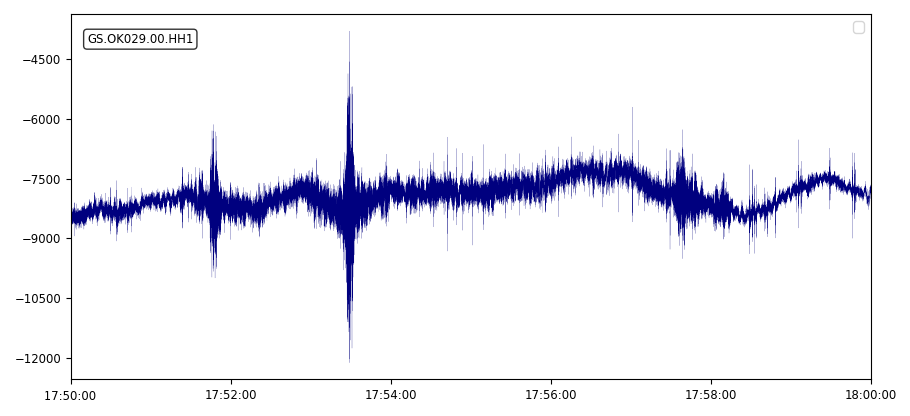
\includegraphics[width=\columnwidth]{../processed-data/10min-example-2018-06-30T17:50.png}
  \caption{10 minute of data example, no earthquake}
	\label{fig:10min-example}
\end{figure}

So the basis for the features is this time serie, for the labels we use a hand-made catalog of earthquake that contains, among other properties, the location, magnitude and time of the earthquake.\newline \newline


Before diving into the machine learning model construction, we have to take care of several difficulties inerrant to the dataset.\newline
First the data collection, after having choosing the location, station and channel from which we want to get the time series we have to download it and store that to a usable format for the next steps. The frequency of the sensors is $100$ data point per second, so the amount of data increase quite quickly. Then, the data has holes in it, the data is missing for some period of time because of casualties or maintenance. Those holes are not regular and unpredictable, so we have to take care of this with caution.

\begin{figure}[h]
  \centering
	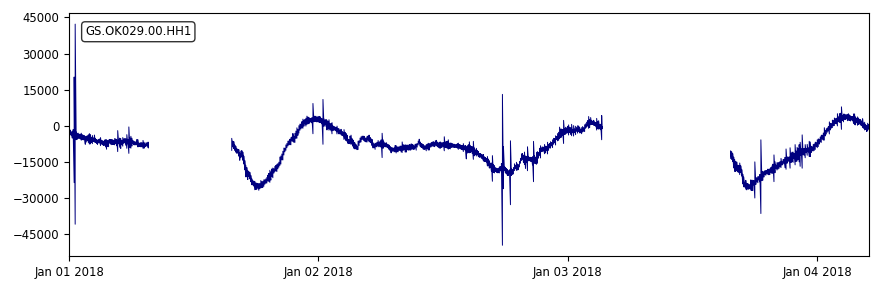
\includegraphics[width=\columnwidth]{../processed-data/hole_example.png}
  \caption{Example of missing values in the dataset}
	\label{fig:10min-example}
\end{figure}

We already mentionned that the data obtained from ObsPy is very noisy, we want to emphasize this and as we will see in examples, some earthquakes and non-earthquakes are undistinguishable for the untrained eye. The catalog is noisy in a sense as well, the time series are parsed by human and thus some earthquakes are missed and as the magnitude decreases the number of missed earthquake increases, being the majority for small magnitudes. Another difficulty in the catalog is the delay that is induced by the difference of location between the detection of the earthquake and the location of our station. All the catalog have to be calibrated to ensure that the time of earthquake corresponds to a peak in our time series.

\section{Data pre-processing}
Develop the pre-processing steps introduced in last section:
- Fill holes in data\\
- Fix delay of catalog\\

\section{Labeling of the Data}
As the dataset live in a continuous space, we have to discretize it. We have to choose time windows that will be classified as earthquake or not earthquake. The choice of the time is crucial and it is hard to predict what would be a good choice. Also, that give rise to a fundamental question for the creation of the labels: when does an earthquake ends? It is possible, in fact rather probable depending on the length of the discretization process, that an earthquake spans over multiple time window thus knowing the duration of the earthquake would permit to overcome this issue. This is important, because not being able to accurately and correctly label our data will of course be disastrous for the machine learning model. Unfortunately, the duration of an earthquake is an open question in geology, the only option simple enough is to label as earthquake only the window that contains the moment of an earthquake.\\
The problem with this approach is illustrated in figure \ref{fig:problem-discretization}. In the catalog the earthquake will be at $T_1$. We can see that the earthquake indeed trigger a big instant augmentation in the variation of the amplitude, that is typical to the earthquakes that are quite easy to classify. The problem here is that when discretizing the time serie in windows, the partitioning of the data will change

\begin{figure}[h]
  \centering
	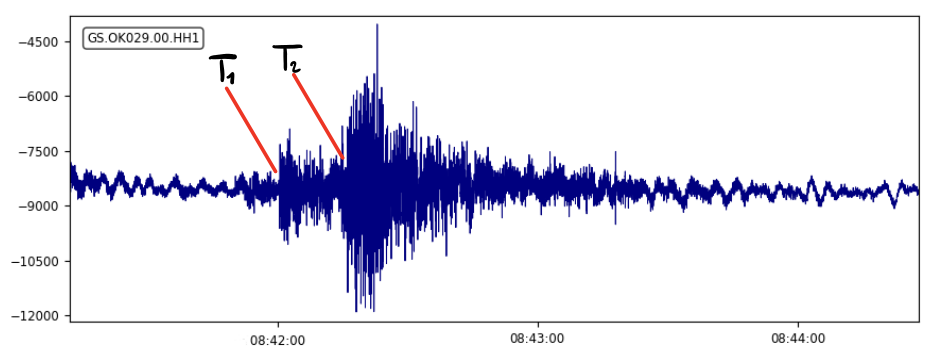
\includegraphics[width=\columnwidth]{../processed-data/problem-time-window-labeling.png}
  \caption{Illustration of the problem of time window labeling}
	\label{fig:problem-discretization}
\end{figure}

\section{Feature Creation}

\section{Model Selection}

\section{Conclusion}

\section{Further improvements}

\begin{thebibliography}{9}
\bibitem{ConNetPaper}
Convolutional neural network for earthquake detection and location, 14 February 2018. \\\texttt{https://advances.sciencemag.org/content/4/2/e1700578}
\bibitem{obspy}
ObsPy: python library to collect seismological data.
\\\texttt{https://docs.obspy.org/}
\end{thebibliography}

\end{document}
